\documentclass[tikz]{standalone}
\usepackage{amsmath, amssymb}
\usetikzlibrary{arrows.meta, shapes.geometric}

\begin{document}
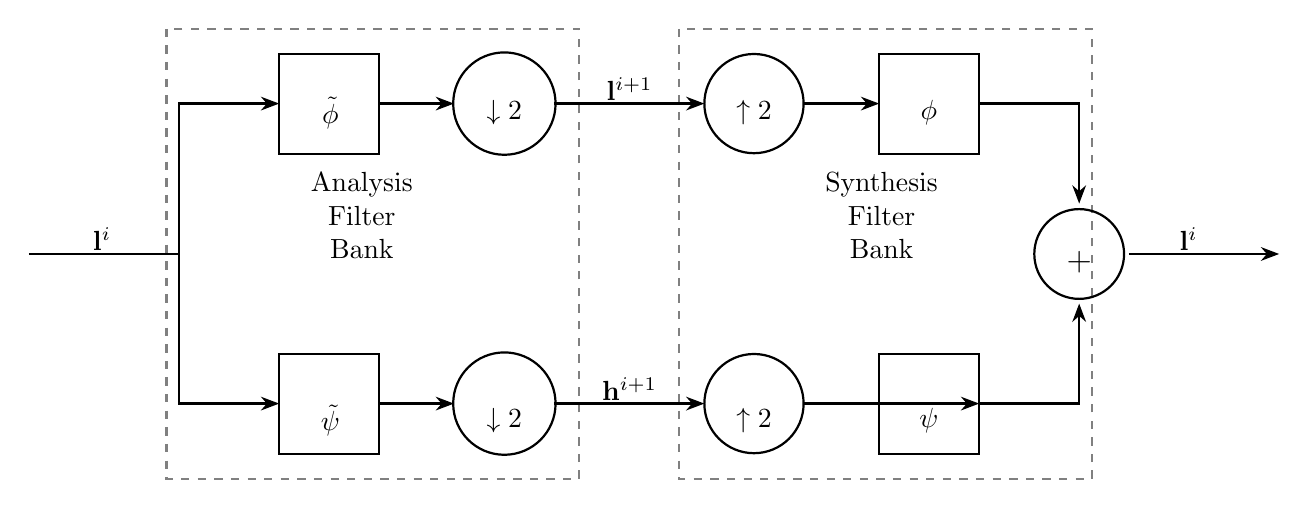
\begin{tikzpicture}[x=1cm, y=-1cm, >=Stealth, thick]
    % Xfig coordinates are scaled: (coord / 1200 * 2.54) to get cm
    % We use y=-1cm because Xfig's origin is top-left

    % --- Boxes (Filters and Processing) ---
    
    % Analysis Filters
    \draw (6.35, 6.35) rectangle (7.62, 7.62); % Analysis Box 1
    \draw (6.35, 10.16) rectangle (7.62, 11.43); % Analysis Box 2
    
    % Synthesis Filters
    \draw (13.97, 6.35) rectangle (15.24, 7.62); % Synthesis Box 1
    \draw (13.97, 10.16) rectangle (15.24, 11.43); % Synthesis Box 2

    % Large Dashed Grouping Boxes
    \draw[dashed, color=gray] (4.92, 6.03) rectangle (10.16, 11.75); % Analysis Bank
    \draw[dashed, color=gray] (11.43, 6.03) rectangle (16.67, 11.75); % Synthesis Bank

    % --- Nodes / Circles (Samplers and Summation) ---
    \draw (9.21, 6.98) circle (0.65); % Downsampler top
    \draw (9.21, 10.79) circle (0.65); % Downsampler bottom
    \draw (12.38, 6.98) circle (0.63); % Upsampler top
    \draw (12.38, 10.79) circle (0.63); % Upsampler bottom
    \draw (16.51, 8.89) circle (0.57); % Summation point

    % --- Polylines (Arrows/Connections) ---
    % Input line branching
    \draw[->] (3.17, 8.89) -- (5.08, 8.89) -- (5.08, 6.98) -- (6.35, 6.98);
    \draw[->] (5.08, 8.89) -- (5.08, 10.79) -- (6.35, 10.79);
    
    % Connections between filters and samplers
    \draw[->] (7.62, 10.79) -- (8.57, 10.79);
    \draw[->] (9.84, 10.79) -- (11.75, 10.79);
    \draw[->] (9.84, 6.98) -- (11.75, 6.98);
    \draw[->] (13.02, 6.98) -- (13.97, 6.98);
    \draw[->] (13.02, 10.79) -- (15.24, 10.79);
    
    % Connections to Summation
    \draw[->] (15.24, 6.98) -- (16.51, 6.98) -- (16.51, 8.25);
    \draw[->] (15.24, 10.79) -- (16.51, 10.79) -- (16.51, 9.52);
    
    % Output line
    \draw[->] (17.14, 8.89) -- (19.05, 8.89);
    
    % Input side labels
    \draw[->] (7.62, 6.98) -- (8.57, 6.98);

    % --- Text Labels ---
    % Titles
    \node at (7.4, 8.4) [align=center] {Analysis\\Filter\\Bank};
    \node at (14.0, 8.4) [align=center] {Synthesis\\Filter\\Bank};

    % Math Labels
    \node at (4.1, 8.7) {${\mathbf l}^i$};
    \node at (17.9, 8.7) {${\mathbf l}^i$};
    \node at (10.8, 6.8) {${\mathbf l}^{i+1}$};
    \node at (10.8, 10.6) {${\mathbf h}^{i+1}$};
    
    \node at (16.51, 9.0) [font=\large] {$+$};
    
    \node at (7.0, 7.1) {$\tilde\phi$};
    \node at (7.0, 11.0) {$\tilde\psi$};
    \node at (14.6, 11.0) {$\psi$};
    \node at (14.6, 7.1) {$\phi$};
    
    \node at (12.38, 7.1) {$\uparrow 2$};
    \node at (12.38, 11.0) {$\uparrow 2$};
    \node at (9.21, 7.1) {$\downarrow 2$};
    \node at (9.21, 11.0) {$\downarrow 2$};

\end{tikzpicture}
\end{document}
